%& /Users/ziky/.cache/org-persist/e7/01d9eb-af3c-4818-9266-4c2a530e1818-832ed4017c79fd5b5d686e66a4a447c3
% Created 2025-11-18 Tue 14:31
% Intended LaTeX compiler: pdflatex
\documentclass[11pt]{article}
\usepackage[utf8]{inputenc}
\usepackage[T1]{fontenc}
\usepackage{amsmath}
\usepackage{amssymb}
\usepackage{capt-of}
\usepackage{hyperref}
\setlength{\abovedisplayskip}{0pt}
\setlength{\belowdisplayskip}{0pt}
\usepackage[a4paper, margin=1in]{geometry}

%% ox-latex features:
%   !announce-start, !guess-pollyglossia, !guess-babel, !guess-inputenc,
%   caption, maths, image, !announce-end.

\usepackage{capt-of}

\usepackage{amsmath}
\usepackage{amssymb}

\usepackage{graphicx}

%% end ox-latex features


% end precompiled preamble
\ifcsname endofdump\endcsname\endofdump\fi

\author{Ziky Zhang}
\date{\today}
\title{Worksheet \#10}
\hypersetup{
 pdfauthor={Ziky Zhang},
 pdftitle={Worksheet \#10},
 pdfkeywords={},
 pdfsubject={},
 pdfcreator={},
 pdflang={English}}
\begin{document}

\maketitle
\begin{enumerate}
\item An electron enters a region of uniform magnetic field and follows the semicircular path shown below before leaving the field \(2.6 \mu \mathrm{s}\) later \(1.4 \mathrm{cm}\) higher than the point where the electron entered the field originally.
\begin{enumerate}
\item How fast is the electron moving?
\item Determine the magnetic field (magnitude and direction) in the region to the left of the dashed line.
\item Suppose that, in addition to the uniform magnetic field, a uniform electric field is also applied to the region to the left of the dashed line, and as a result, the electron no longer deflects. Determine this electric field (magnitude and direction).
\begin{figure}[htbp]
\centering
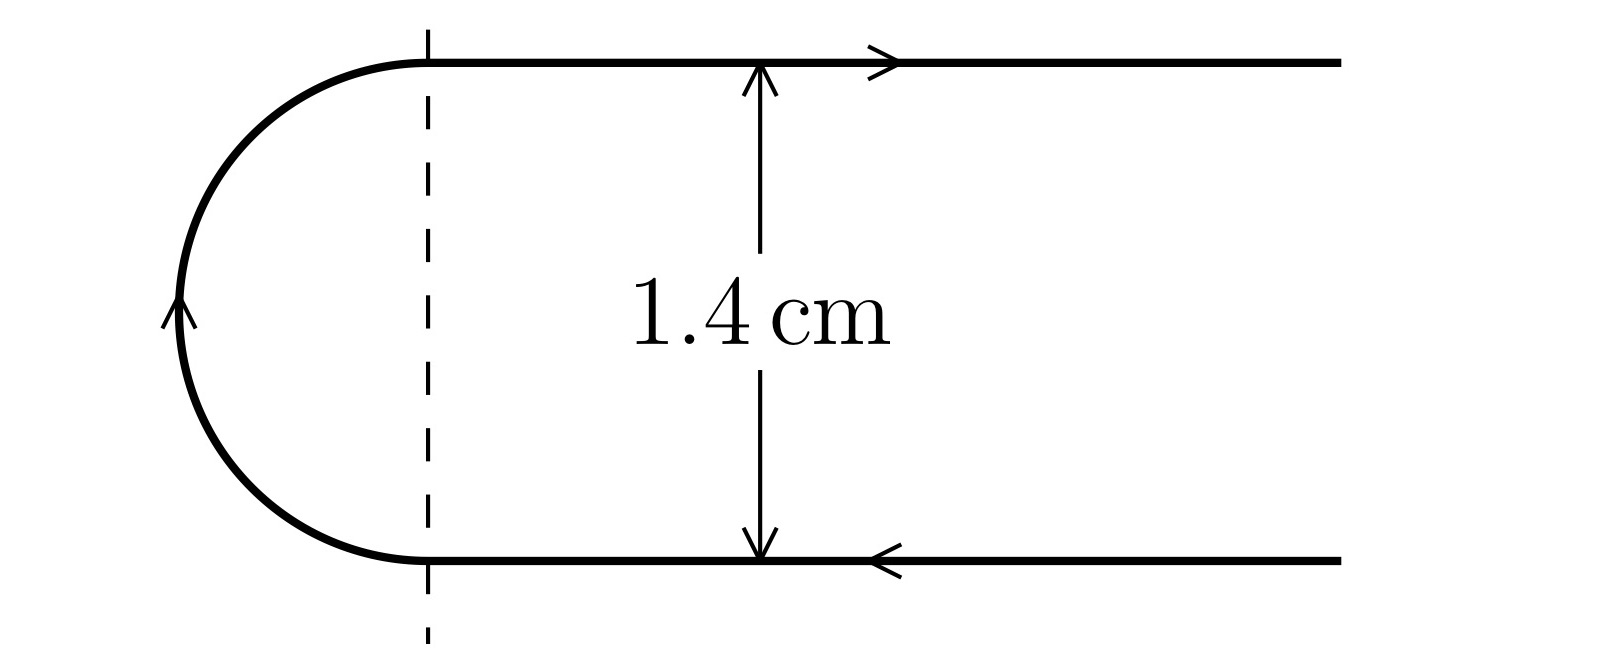
\includegraphics[height=3cm]{./img/10.1.jpg}
\caption{\label{fig:org7e89cf9}Semi-circular path of electron}
\end{figure}
\end{enumerate}

\item A \(3.0 \mathrm{m} \times 1.0 \mathrm{cm} \times 0.10 \mathrm{mm}\) rectangular slab carrying a \(67 \mathrm{mA}\) current to the right is placed in a uniform magnetic field of \(34 \mathrm{mT}\), directed upward. The rectangular slab is made of an unknown (semi-conducting) substance. A voltmeter is connected across the width of the circuit, as shown below, and reads \(+4.6 \mathrm{mV}\).
\begin{center}
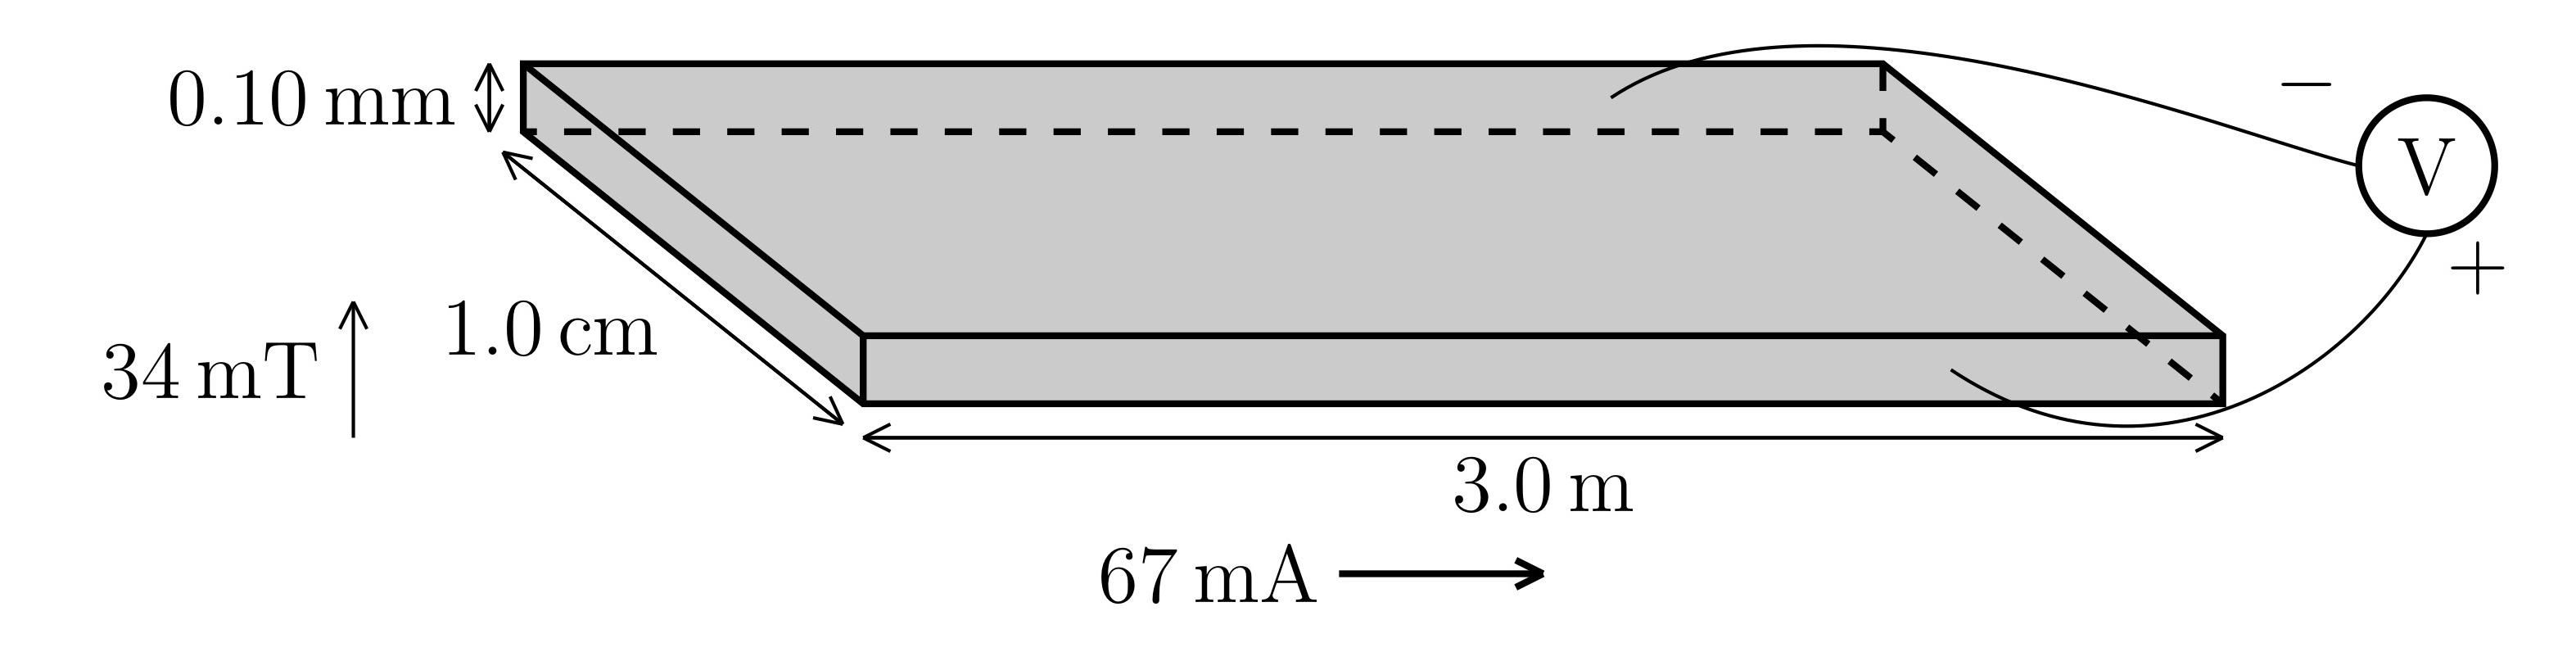
\includegraphics[width=.9\linewidth]{./img/10.2.jpg}
\end{center}
\begin{enumerate}
\item Are the current-carrying charges positive or negative? Explain your reasoning.
\item Calculate the number density of current-carrying chargees (assume each charge is \(\pm e\)).
\end{enumerate}
\end{enumerate}

\newpage
\begin{enumerate}
\item 
\end{enumerate}

\begin{align*}
\text{Variables:} \\
\text{Direction of motion} &\text{: clockwise} \\
m_{\mathrm{e}} &= 9.11 \times 10^{-31} kg \\
q_{\mathrm{e}} &= e^- = 1.60 \times 10^{-19} \mathrm{C}\\
\Delta h &= 1.4 \mathrm{cm} = 1.4 \times 10^{-2} \mathrm{m} \\
\Delta t &= 2.6 \mu \mathrm{s} = 2.6 \times 10^{-6} \mathrm{s} \\
r &= 0.7 \mathrm{cm} = 7 \times 10^{-3} \mathrm{m}
\end{align*}

1.(a)
\begin{align*}
v &= \pi r / t \\
  &= 7 \times 10^{-3} \mathrm{m} \pi / 2.6 \times 10^{-6} \mathrm{s} \\
  &= \frac{21.99 \times 10^{-3} \mathrm{m}}{2.6 \times 10^{-6} \mathrm{s}} \\
  &= 8.458 \times 10^3 \mathrm{m / s}
\end{align*}

1.(b)
\begin{align*}
|q|vB &= \frac{mv^2}{r} \\
B &= \frac{m_{\mathrm{e}}v^2}{|q|rv} \\
  &= \frac{(9.11 \times 10^{-31} \mathrm{kg}) (8.458 \times 10^3 \mathrm{m / s})}{(1.60 \times 10^{-19} \mathrm{C}) (7 \times 10^{-3} \mathrm{m})} \\
  &= \frac{77.05 \times 10^{-28} \mathrm{kg \ m / s}}{11.2 \times 10^{-22} \mathrm{C\ m}} \\
  &= - 6.879 \times 10^{-6} \mathrm{T} \ (\hat{k}) \text{ into the page}
\end{align*}


1.(c)
\begin{align*}
\begin{aligned}[t]
\overrightarrow{F_{\mathrm{B}}} &= q \cdot \overrightarrow{v} \times \overrightarrow{B} \\
  &= q\cdot [8.458 \times 10^3 \mathrm{m/s} \ (-\hat{i}) \times - 6.879 \times 10^{-6} \mathrm{T} \ (\hat{k})] \\
  &= - 1.60 \times 10^{-19} \mathrm{C} \cdot - 58.18 \times 10^{-3} \mathrm{T\ m/s} \ (\hat{j}) \\
  &= 93.09 \times 10^{-22} \mathrm{N} \ (\hat{j})
\end{aligned}
\quad
\begin{aligned}[t]
\overrightarrow{F_{\mathrm{E}}} &= - \overrightarrow{F_{\mathrm{B}}} \\
\overrightarrow{E} &= \frac{- \overrightarrow{F_{\mathrm{B}}}}{q} \\
  &= \frac{- \overrightarrow{F_{\mathrm{B}}}}{q} \\
  &= \frac{- 93.09 \times 10^{-22} \mathrm{N} \ (\hat{j})}{- 1.60 \times 10^{-19} \mathrm{C}} \\
  &= 5.818125 \times 10^{-2} \mathrm{N/C} \ ({\hat{j}}) \text{ upwards}
\end{aligned}
\end{align*}

\newpage
2.(a)
Let \(+\hat{k}\) be the direction magnetic field is point towards, \(+\hat{i}\) is the direction current is drifting towards, then positive side of the voltmeter is hooked onto the \(+\hat{j}\) side and negative side of the voltmeter is hooked onto the \(-\hat{j}\) side.
\begin{align*}
\overrightarrow{v_{\mathrm{drift}}} \times \overrightarrow{B} &= \hat{i} \times \hat{k} \\
  &= -\hat{j}
\end{align*}
with the calculation above, we learn that if the current is carrying positive charges, the sign will stay the same and voltmeter will read a negative value. So the charges the current is carrying must be negative.

2.(b)
\begin{align*}
\begin{aligned}[t]
\text{Variables: }
I &=67.0\ \mathrm{mA}=6.7 \times 10^{-2}\mathrm{A} \\
B & =34.0\ \mathrm{mT}=3.4 \times 10^{-2}\mathrm{T} \\
h & =0.10\ \mathrm{mm}=1.0 \times 10^{-4}\mathrm{m} \\
V_\mathrm{H} & =4.6\ \mathrm{mV}=4.6 \times 10^{-3}\mathrm{V} \\
e &=1.602 \times 10^{-19}\mathrm{C}
\end{aligned}
\quad
\begin{aligned}[t]
V_{\mathrm{H}} &= \frac{I B}{n q A} w \\
  &= \frac{I B}{nqh} \\
n &= \frac{I B}{qh V_\mathrm{H}} \\
  &=\frac{(6.7 \times 10^{-2} \mathrm{A}) (3.4 \times 10^{-2} \mathrm{T})}{(1.602 \times 10^{-19} \mathrm{C})(1.0 \times 10^{-4} \mathrm{m})(4.6 \times 10^{-3}) \mathrm{V}} \\
  &\approx 3.09\times10^{22}\ \mathrm{m^{-3}}
\end{aligned}
\end{align*}
\end{document}
